% !TeX root = surprises.tex

\selectlanguage{hebrew}
\chapter{הבעיה של 
\L{Langford}}
\label{c.langford}

המתמטיקאי
\L{C. Dudley Langford}
שם לב שבנו סידר קוביות צבעוניות לפי הסדר:
\begin{center}
\selectlanguage{english}
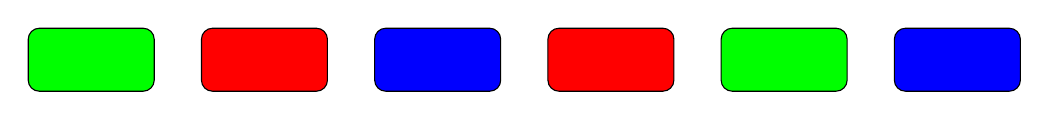
\begin{tikzpicture}
\draw[rounded corners,fill=green] (0,0)  
  rectangle +(1.6cm,.8cm);
\draw[rounded corners,fill=red]   (2.2,0)
  rectangle +(1.6cm,.8cm);
\draw[rounded corners,fill=blue]  (4.4,0)
  rectangle +(1.6cm,.8cm);
\draw[rounded corners,fill=red]   (6.6,0)
  rectangle +(1.6cm,.8cm);
\draw[rounded corners,fill=green] (8.8,0)
  rectangle +(1.6cm,.8cm);
\draw[rounded corners,fill=blue]  (11,0)
  rectangle +(1.6cm,.8cm);
\end{tikzpicture}
\end{center}

קוביה אחת נמצאת בין שתי הקוביות האדומות, שתי קוביות בין הקוביות הכחולות, ושלוש קוביות בין הקוביות הירוקות. ניתן לנסח את הבעיה כך:
נתון שק%
\footnote{
שק הוא  קבוצה בה איבר יכול להופיע מספר פעמים.} של מספרים
$\{1,1,2,2,3,3\}$,
האם אפשר לסדר אותם בסדרה כך שלכל
$1\leq i \leq 3$,
$i$
מספרים נמצאים בין שני המופעים של
$i$?

\textbf{
הבעיה של
\L{Langford} $L(n)$}:
נתון שק של מספרים
$\{1,1,2,2,3,3,\ldots,n,n\}$,
האם ניתן לסדר אותם כך שלכל
$1\leq i \leq n$, $i$
מספרים נמצאים בין שני המופעים של
$i$?


מהאיור לעיל אנו רואים שעבור 
$n=3$
הפתרון הוא
$312132$.


%%%%%%%%%%%%%%%%%%%%%%%%%%%%%%%%%%%%%%%%%%%%%%

\section{
הבעיה של
\L{Langford}
כבעיית כיסוי}

ניתן להציג את הבעיה של
\L{Langford}
באמצעות טבלה. עבור
$L(3)$
יש
$6$
עמודות, אחת לכל מקום בסדרה. השורות מציגות את כל האפשרויות לסדר את  שני המופעים של המספרים. קל לראות שיש ארבעה זוגות של מקומות אפשריים עבור
$1$,
שלושה עבור
$2$
ושניים עבור
$3$:
%)טבלה~%
%\ref{t.lang3:1}(.

%\begin{table}
\[
\erh{2pt}
\begin{array}{|c||c|c|c|c|c|c|}
\hline
&1&2&3&4&5&6\\\hline\hline
1&1&&1&&&\\\hline
2&&1&&1&&\\\hline
3&&&1&&1&\\\hline
4&&&&1&&1\\\hline
5&2&&&2&&\\\hline
6&&2&&&2&\\\hline
7&&&2&&&2\\\hline
8&3&&&&3&\\\hline
9&&3&&&&3\\\hline
\end{array}
\]
%\caption{סידורים אפשריים}\label{t.lang3:1}
%\end{table}


כדי לפתור את הבעיה, עלינו לבחור שורה אחת עבור המופעים של
$1$,
שורה אחת עבור המופעים של
$2$
ושורה אחת עבור המופעים של
$3$,
כך שאם הנמקם את השורות אחת מעל לשניה, בכל עמודה יש רק מספר אחד: 
%)טבלה~%
%\ref{t.lang3:2}(.

%\begin{table}[H]
\[
\erh{2pt}
\begin{array}{|c||c|c|c|c|c|c|}
\hline
&1&2&3&4&5&6\\\hline\hline
2&&1&&1&&\\\hline
7&&&2&&&2\\\hline
8&3&&&&3&\\\hline
\end{array}
\]
%\caption{סידור סופי}\label{t.lang3:2}
%\end{table}


שורה
$9$
אינה נחוצה בגלל סימטריה: סדרה המתחילה עם השורה
$9$
זהה לסדרה מתקבלת מהפיכת הסדר של סדרה המתקבלת כאשר מתחילים עם שורה
$8$.

שורה 
$8$
היא היחידה המכילה את המספר
$3$
כך שחובה לבחור אותה, והסדרה המתקבלת היא
\L{3\textvisiblespace \textvisiblespace \textvisiblespace 3\textvisiblespace}. 
אי אפשר להשתמש בכל שורה שיש לה מספרים בעמודות
$1$
ו-
$5$,
כי מותר רק מספר אחד בכל מקום. נסמן את השורות שניתן לבחור ושלא ניתן לבחור כך:
$\not 1,2,\not 3,4,\not 5, \not 6, 7, 8$.

שורה
$7$
היא השורה האפשרית היחידה עבור
$2$
כך שחובה לבחור בה והתוצאה היא
\L{3\textvisiblespace 2\textvisiblespace 3{}2}.
נעדכן את רשימת השורות ונקבל:
$\not 1,2,\not 3,\not 4,\not 5, \not 6, 7, 8$.

כעת, ניתן לבחור רק שורה
$2$
ומתקבל הפתרון
$3{}1{}2{}1{}3{}2$.

טבלה~%
~\ref{t.lang4}
היא הטבלה עבור
$L(4)$.
הפתרון הוא
$41312432$.

\begin{table}
\[
\erh{-2pt}
\begin{array}{|c||c|c|c|c|c|c|c|c|}
\hline
&1&2&3&4&5&6&7&8\\\hline\hline
1&1&&1&&&&&\\\hline
2&&1&&1&&&&\\\hline
3&&&1&&1&&&\\\hline
4&&&&1&&1&&\\\hline
5&&&&&1&&1&\\\hline
6&&&&&&1&&1\\\hline
7&2&&&2&&&&\\\hline
8&&2&&&2&&&\\\hline
9&&&2&&&2&&\\\hline
10&&&&2&&&2&\\\hline
11&&&&&2&&&2\\\hline
12&3&&&&3&&&\\\hline
13&&3&&&&3&&\\\hline
14&&&3&&&&3&\\\hline
15&&&&3&&&&3\\\hline
16&4&&&&&4&&\\\hline
17&&4&&&&&4&\\\hline
18&&&4&&&&&4\\\hline
\end{array}
\]
\caption{הבעיה של
\L{Langford}
$L(4)$}\label{t.lang4}
\end{table}


\section{
עבור איזה ערכים של
$n$
ניתן לפתור את הבעיה}
\begin{theorem}\mbox{}\\
ניתן למצוא פתרון ל-%
$L(n)$
אם ורק אם
$n=4k$
או
$n=4k-1$.
\end{theorem}
נוכיח רק שאם 
$n=4k-2$
או
$n=4k-3$
אין פתרון לבעיה.

\textbf{הוכחה 1}

אם המופע הראשון של המספר
$k$
נמצא במקום
$i_k$,
המופע השני נמצא במקום
$i_k+k+1$.
לכן,
$S_n$,
סכום המקומות של כל המספרים, הוא:
\erh{8pt}
\begin{equationarray*}{rcl}
S_n&=&\sum_{k=1}^{n}i_k+\sum_{k=1}^{n}(i_k+k+1)\\
& =& 2\sum_{k=1}^{n}i_k+\sum_{k=1}^{n}(k+1)\\
&=& 2\sum_{k=1}^{n}i_k+\frac{n(n+3)}{2}\,.
\end{equationarray*}
אבל
$S_n$
הוא פשוט
$1+2+3+\cdots+2n$
ולפי הנוסחה לסיכום סדרת מספרים:
\[
S_n=\sum_{k=1}^{2n}k = \frac{2n(2n+1)}{2}\,.
\]
נשווה את שני הביטויים עבור
$S_n$:
\erh{8pt}
\begin{equationarray*}{rcl}
2\sum_{k=1}^{n}i_k+\frac{n(n+3)}{2} &=& \frac{2n(2n+1)}{2}\\
\sum_{k=1}^{n}i_k &=& \frac{1}{2}\left(\frac{2n(2n+1)}{2} - \frac{n(n+3)}{2}\right) \\
&=& \frac{3n^2-n}{4}\,.
\end{equationarray*}

הצד השמאלי חייב להיות מספר שלם כי הוא סכום של מספרים שלמים. לכן, הצד הימני חייב גם הוא להיות מספר שלם, כלומר,
$3n^2-n=n(3n-1)$
חייב להתחלק ב-%
$4$.
\begin{itemize}
\item
אפשרות אחת היא ש-%
$n$
בעצמו מתחלק ב-%
$4$.
\item

מתי 
$3n-1$
מתחלק ב-%
$4$?
ניתן להציג את
$n$
כ-%
$n=4i+j$
עבור
$j=0,1,2,3$.
אם 
$3n-1$
מתחלק ב-%
$4$,
גם
$3(4i+j)-1 = 12i+3j-1$
מתחלק ב-%
$4$.
$12i$
מתחלק ב-%
$4$,
וקל לראות ש-%
$3j-1$
מתחלק ב-%
$4$
)עבור 
$j=0,1,2,3$%
( רק אם
$j=3$.
מכאן ש-%
$3n-1$
מתחלק ב-%
$4$
רק עבור
$n=4i+3=4(i+1)-1=4k-1$.
\end{itemize}
\qed

\newpage

\textbf{הוכחה
\L{2}}


נעיין בפתרון עבור
$n=4$
ונבדוק תחילה את מקומות המופעים של המספרים הזוגיים:
\[
\erh{-2pt}
\begin{array}{|c|c|c|c|c|c|c|c|}
\hline
1&2&3&4&5&6&7&8\\
\hline\hline
4&1&3&1&2&4&3&2\\\hline
*&&&&&*&&\\\hline
\end{array}
\hspace{3em}
\begin{array}{|c|c|c|c|c|c|c|c|}
\hline
1&2&3&4&5&6&7&8\\
\hline\hline
4&1&3&1&2&4&3&2\\\hline
&&&&*&&&*\\\hline
\end{array}
\]
מקומות המופעים של
$4$
הם
$1$
ו-%
$6$,
ומקומות המופעים של
$2$
הם
$5$
ו-%
$8$.
ניקח מספר
\textbf{זוגי}
$k=2m$. 
מקום המופע הראשון שלו הוא
$i$
ומקום המופע השני שלו הוא
$i+k+1$.
סכום המקומות הוא:
\[
i+(i+k+1)=2i+2m+1=2(i+m)+1
\]
שהוא מספר אי-זוגי.
סכום של שני מספרים הוא אי-זוגיים אם ורק אם אחד זוגי והשני אי-זוגי.

נבדוק עכשיו את מקומות המופעים של המספרים האי-זוגיים:

\[
\erh{-2pt}
\begin{array}{|c|c|c|c|c|c|c|c|}
\hline
1&2&3&4&5&6&7&8\\
\hline\hline
4&1&3&1&2&4&3&2\\\hline
&*&&*&&&&\\\hline
\end{array}
\hspace{3em}
\begin{array}{|c|c|c|c|c|c|c|c|}
\hline
1&2&3&4&5&6&7&8\\
\hline\hline
4&1&3&1&2&4&3&2\\\hline
&&*&&&&*&\\\hline
\end{array}
\]
מקומות המופעים של
$1$
הם
$2$
ו-%
$4$,
ומקומות המופעים של
$3$
הם
$3$
ו-%
$7$.
ניקח מספר 
\textbf{אי-זוגי},
$k=2m+1$.
מקום המופע הראשון שלו הוא
$i$
ומקום המופע השני שלו הוא
$i+k+1$.
סכום המקומות הוא:
\[
i+(i+k+1)=2i+2m+1+1=2(i+m+1)\,,
\]
שהוא מספר זוגי.
סכום של שני מספרים הוא זוגי אם ורק אם שניהם זוגיים או שניהם אי-זוגיים.

ברור שרשימת המקומות של המספרים בסדרה,
$1,2,\ldots,2n-1,2n$,
מכילה מספר שווה של מקומות זוגיים ומקומות אי-זוגיים. כאשר מציבים את שני המופעים של מספר בסדרה, הם "תופסים" שני מקומות. כאשר מסיימים להציב את כל המספרים בפתרון, חייבים להיות מספר שווה של מקומות זוגיים ואי-זוגיים "שנתפסו".

\textbf{זוגיות}
היא ההפרש בין מספר המקומות הזוגיים שנתפסו לבין מספר המקומות האי-זוגיים שנתפסו. תחילה הזוגיות היא אפס, ואם יש פתרון זוגיות שלו גם כן אפס. אנו נמצא את התנאים על 
$n$ 
כך שהזוגיות לא תתאפס. עבור ערכים אלה אין פתרון.

כאשר ממקמים את שני המופעים של מספר זוגי, הם תופסים מקום אחד זוגי )מסומן 
$+1$(
ומקום אחר אי-זוגי )מסומן 
$-1$(,
וסכום הזוגיות הוא אפס.

\[
\erh{-2pt}
\begin{array}{|c|c|c|c|c|c|c|c|}
\hline
1&2&3&4&5&6&7&8\\
\hline\hline
4&1&3&1&2&4&3&2\\\hline
-1&&&&&+1&&\\\hline
\end{array}
\hspace{3em}
\begin{array}{|c|c|c|c|c|c|c|c|}
\hline
1&2&3&4&5&6&7&8\\
\hline\hline
4&1&3&1&2&4&3&2\\\hline
&&&&-1&&&+1\\\hline
\end{array}
\]

כאשר ממקמים את שני המופעים של מספר אי-זוגי,  הם תופסים שני מקומות זוגיים )מסומן 
$+1$(
או שני מקומות אי-זוגיים )מסומן 
$-1$(,
וסכום הזוגיות היא
$\pm 2$.
\[
\erh{-2pt}
\begin{array}{|c|c|c|c|c|c|c|c|}
\hline
1&2&3&4&5&6&7&8\\
\hline\hline
4&1&3&1&2&4&3&2\\\hline
&+1&&+1&&&&\\\hline
\end{array}
\hspace{3em}
\begin{array}{|c|c|c|c|c|c|c|c|}
\hline
1&2&3&4&5&6&7&8\\
\hline\hline
4&1&3&1&2&4&3&2\\\hline
&&-1&&&&-1&\\\hline
\end{array}
\]
כדי שהזוגיות תתאפס
\textbf{חייב להיות מספר זוגי של מספרים אי-זוגיים ב}-%
$\{1,\ldots,n\}$!
נוכיח שאם 
$n=4k, 4k\!-\!1$
יש מספר זוגי של אי-זוגיים )וכנראה שיש פתרון(,
ואם
$n=4k\!-\!2, 4k\!-\!3$
יש מספר אי-זוגי של אי-זוגיים )ואין פתרון(.

ההוכחה באינדוקציה. עבור 
$k=1$:
\begin{itemize}
\item $n=4k-3=1$.
ב-%
$\{1\}$
יש מספר אי-זוגי של אי-זוגיים )וברור שאין פתרון(.
\item $n=4k-2=2$.
ב-%
$\{1,2\}$
יש מספר אי-זוגי של אי-זוגיים )וברור שאין פתרון(.
\item $n=4k-1=3$.
ב-%
$\{1,2,3\}$
יש מספר זוגי של אי-זוגיים )וראינו שיש פתרון(.
\item $n=4k-0=4$.
ב-%
$\{1,2,3,4\}$
יש מספר זוגי של אי-זוגיים )וראינו שיש פתרון(.
\end{itemize}

נניח שהטענה נכונה עבור 
$n=4k-j, k\geq 1, 0\leq j\leq 3$,
ונוכיח שהטענה נכונה עבור
$n=4(k+1)-j, k\geq 1, 0\leq j\leq 3$.
\begin{itemize}
\item
נוסיף לשק את המספר הבא אחרי 
$4k$
שהוא
$4k+1=4(k+1)-3$.
לפי הנחת האינדוקציה עבור  
$n=4k-0$
יש מספר זוגי של אי-זוגיים. 
$4(k+1)-3$
הוא אי-זוגי ולכן יש עכשיו מספר אי-זוגי של אי-זוגיים )אין פתרון(.

\item
נוסיף לשק את המספר הבא אחרי 
$4k+1$
שהוא
$4k+2=4(k+1)-2$.
הוכחנו שעבור
$n=4k+1$
יש מספר אי-זוגי של אי-זוגיים. 
$4(k+1)-2$
הוא זוגי ולכן עדיין יש מספר אי-זוגי של אי-זוגיים )אין פתרון(.

\item
נוסיף לשק את המספר הבא אחרי 
$4k+2$
שהוא
$4k+3=4(k+1)-1$.
הוכחנו שעבור
$n=4k+2$
יש מספר אי-זוגי של אי-זוגיים. 
$4(k+1)-1$
הוא אי-זוגי ולכן עכשיו יש מספר זוגי של אי-זוגיים )כנראה שיש פתרון(.

\item
נוסיף לשק את המספר הבא אחרי 
$4k+3$
שהוא
$4k+4=4(k+1)-0$.
הוכחנו שעבור
$n=4k+3$
יש מספר זוגי של אי-זוגיים. 
$4(k+1)-0$
הוא זוגי ולכן עדיין יש מספר זוגי של אי-זוגיים )כנראה שיש פתרון(.

\end{itemize}

\vspace{-2ex}

\subsection*{מקורות}
פרק זה מבוסס על
\L{\cite{miller}}.
\L{Davies}
מראה איך למצוא פתרון כאשר הזוגיות היא אפס.
